\documentclass[]{article}
\usepackage{lmodern}
\usepackage{amssymb,amsmath}
\usepackage{ifxetex,ifluatex}
\usepackage{fixltx2e} % provides \textsubscript
\ifnum 0\ifxetex 1\fi\ifluatex 1\fi=0 % if pdftex
  \usepackage[T1]{fontenc}
  \usepackage[utf8]{inputenc}
\else % if luatex or xelatex
  \ifxetex
    \usepackage{mathspec}
    \usepackage{xltxtra,xunicode}
  \else
    \usepackage{fontspec}
  \fi
  \defaultfontfeatures{Mapping=tex-text,Scale=MatchLowercase}
  \newcommand{\euro}{€}
\fi
% use upquote if available, for straight quotes in verbatim environments
\IfFileExists{upquote.sty}{\usepackage{upquote}}{}
% use microtype if available
\IfFileExists{microtype.sty}{%
\usepackage{microtype}
\UseMicrotypeSet[protrusion]{basicmath} % disable protrusion for tt fonts
}{}
\usepackage[margin=1in]{geometry}
\usepackage{color}
\usepackage{fancyvrb}
\newcommand{\VerbBar}{|}
\newcommand{\VERB}{\Verb[commandchars=\\\{\}]}
\DefineVerbatimEnvironment{Highlighting}{Verbatim}{commandchars=\\\{\}}
% Add ',fontsize=\small' for more characters per line
\usepackage{framed}
\definecolor{shadecolor}{RGB}{248,248,248}
\newenvironment{Shaded}{\begin{snugshade}}{\end{snugshade}}
\newcommand{\KeywordTok}[1]{\textcolor[rgb]{0.13,0.29,0.53}{\textbf{{#1}}}}
\newcommand{\DataTypeTok}[1]{\textcolor[rgb]{0.13,0.29,0.53}{{#1}}}
\newcommand{\DecValTok}[1]{\textcolor[rgb]{0.00,0.00,0.81}{{#1}}}
\newcommand{\BaseNTok}[1]{\textcolor[rgb]{0.00,0.00,0.81}{{#1}}}
\newcommand{\FloatTok}[1]{\textcolor[rgb]{0.00,0.00,0.81}{{#1}}}
\newcommand{\CharTok}[1]{\textcolor[rgb]{0.31,0.60,0.02}{{#1}}}
\newcommand{\StringTok}[1]{\textcolor[rgb]{0.31,0.60,0.02}{{#1}}}
\newcommand{\CommentTok}[1]{\textcolor[rgb]{0.56,0.35,0.01}{\textit{{#1}}}}
\newcommand{\OtherTok}[1]{\textcolor[rgb]{0.56,0.35,0.01}{{#1}}}
\newcommand{\AlertTok}[1]{\textcolor[rgb]{0.94,0.16,0.16}{{#1}}}
\newcommand{\FunctionTok}[1]{\textcolor[rgb]{0.00,0.00,0.00}{{#1}}}
\newcommand{\RegionMarkerTok}[1]{{#1}}
\newcommand{\ErrorTok}[1]{\textbf{{#1}}}
\newcommand{\NormalTok}[1]{{#1}}
\usepackage{graphicx}
\makeatletter
\def\maxwidth{\ifdim\Gin@nat@width>\linewidth\linewidth\else\Gin@nat@width\fi}
\def\maxheight{\ifdim\Gin@nat@height>\textheight\textheight\else\Gin@nat@height\fi}
\makeatother
% Scale images if necessary, so that they will not overflow the page
% margins by default, and it is still possible to overwrite the defaults
% using explicit options in \includegraphics[width, height, ...]{}
\setkeys{Gin}{width=\maxwidth,height=\maxheight,keepaspectratio}
\ifxetex
  \usepackage[setpagesize=false, % page size defined by xetex
              unicode=false, % unicode breaks when used with xetex
              xetex]{hyperref}
\else
  \usepackage[unicode=true]{hyperref}
\fi
\hypersetup{breaklinks=true,
            bookmarks=true,
            pdfauthor={Kim Monks},
            pdftitle={Reproducible Research: Peer Assessment 1},
            colorlinks=true,
            citecolor=blue,
            urlcolor=blue,
            linkcolor=magenta,
            pdfborder={0 0 0}}
\urlstyle{same}  % don't use monospace font for urls
\setlength{\parindent}{0pt}
\setlength{\parskip}{6pt plus 2pt minus 1pt}
\setlength{\emergencystretch}{3em}  % prevent overfull lines
\setcounter{secnumdepth}{0}

%%% Use protect on footnotes to avoid problems with footnotes in titles
\let\rmarkdownfootnote\footnote%
\def\footnote{\protect\rmarkdownfootnote}

%%% Change title format to be more compact
\usepackage{titling}
\setlength{\droptitle}{-2em}
  \title{Reproducible Research: Peer Assessment 1}
  \pretitle{\vspace{\droptitle}\centering\huge}
  \posttitle{\par}
  \author{Kim Monks}
  \preauthor{\centering\large\emph}
  \postauthor{\par}
  \predate{\centering\large\emph}
  \postdate{\par}
  \date{Wednesday, August 05, 2015}




\begin{document}

\maketitle


\subsection{Loading and preprocessing the
data}\label{loading-and-preprocessing-the-data}

\subsection{What is mean total number of steps taken per
day?}\label{what-is-mean-total-number-of-steps-taken-per-day}

\subsection{What is the average daily activity
pattern?}\label{what-is-the-average-daily-activity-pattern}

\subsection{Imputing missing values}\label{imputing-missing-values}

\subsection{Are there differences in activity patterns between weekdays
and
weekends?}\label{are-there-differences-in-activity-patterns-between-weekdays-and-weekends}

\section{Reproducible Research: Peer Assessment
1}\label{reproducible-research-peer-assessment-1}

\subsection{Loading and preprocessing the
data}\label{loading-and-preprocessing-the-data-1}

\begin{Shaded}
\begin{Highlighting}[]
\KeywordTok{library}\NormalTok{(ggplot2)}
\KeywordTok{library}\NormalTok{(plyr)}
\KeywordTok{unzip}\NormalTok{(}\StringTok{"./activity.zip"}\NormalTok{) }
\NormalTok{raw.activity <-}\StringTok{ }\KeywordTok{read.csv}\NormalTok{(}\StringTok{"./activity.csv"}\NormalTok{)}
\end{Highlighting}
\end{Shaded}

\section{For this part of the assignment, you can ignore the missing
values in the
dataset}\label{for-this-part-of-the-assignment-you-can-ignore-the-missing-values-in-the-dataset}

\begin{Shaded}
\begin{Highlighting}[]
\NormalTok{activity <-}\StringTok{ }\NormalTok{raw.activity[}\KeywordTok{complete.cases}\NormalTok{(raw.activity),]  }
\end{Highlighting}
\end{Shaded}

\subsection{What is mean total number of steps taken per
day?}\label{what-is-mean-total-number-of-steps-taken-per-day-1}

\subsection{1.Make a histogram of the total number of steps taken each
day}\label{make-a-histogram-of-the-total-number-of-steps-taken-each-day}

\begin{Shaded}
\begin{Highlighting}[]
\NormalTok{steps <-}\StringTok{ }\KeywordTok{tapply}\NormalTok{(activity$steps, activity$date, sum)}
\KeywordTok{qplot}\NormalTok{(steps) +}\StringTok{ }\KeywordTok{geom_histogram}\NormalTok{(}\DataTypeTok{colour=}\StringTok{"black"}\NormalTok{, }\DataTypeTok{fill=}\StringTok{"grey"}\NormalTok{) +}\StringTok{ }
\StringTok{  }\KeywordTok{labs}\NormalTok{(}\DataTypeTok{x=}\StringTok{"Steps per day"}\NormalTok{, }\DataTypeTok{y=}\StringTok{"Frequency"}\NormalTok{, }\DataTypeTok{title=}\StringTok{"Histogram of total steps per day"}\NormalTok{)}
\end{Highlighting}
\end{Shaded}

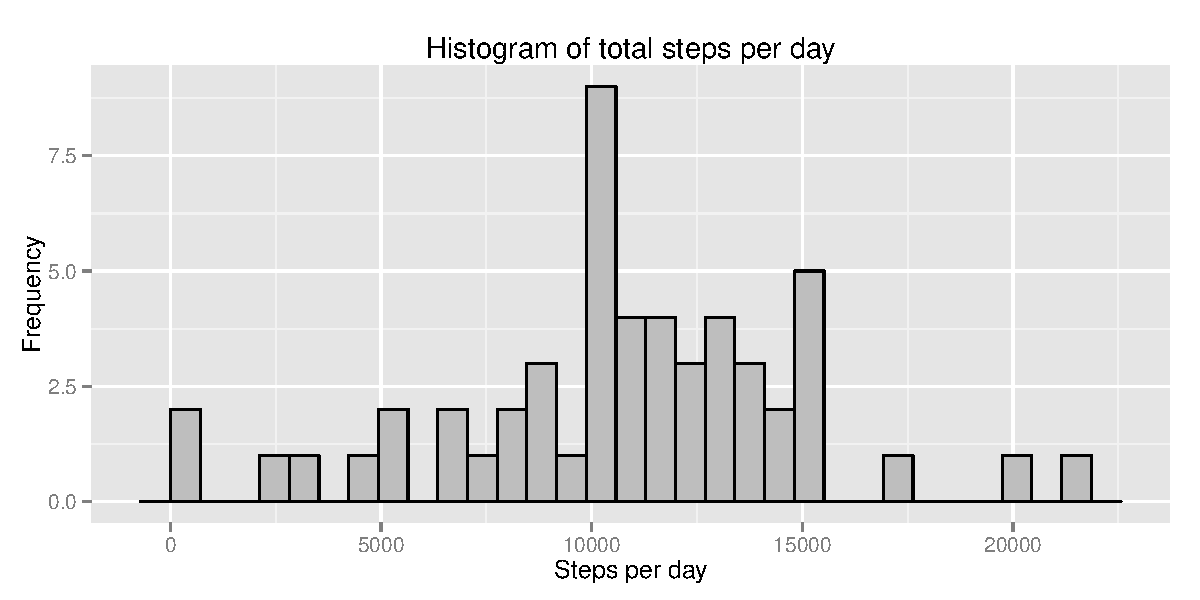
\includegraphics{PA1_template_files/figure-latex/unnamed-chunk-3-1.pdf}

\subsection{2.Calculate and report the mean and median total number of
steps taken per
day}\label{calculate-and-report-the-mean-and-median-total-number-of-steps-taken-per-day}

\begin{Shaded}
\begin{Highlighting}[]
\NormalTok{mean.steps <-}\StringTok{ }\KeywordTok{mean}\NormalTok{(steps, }\DataTypeTok{na.rm=}\OtherTok{TRUE}\NormalTok{)}
\NormalTok{median.steps <-}\StringTok{ }\KeywordTok{median}\NormalTok{(steps, }\DataTypeTok{na.rm=}\OtherTok{TRUE}\NormalTok{)}
\end{Highlighting}
\end{Shaded}

The mean number of total steps per day is
\textbf{1.0766189\times 10\^{}\{4\}} and the median is \textbf{10765}.

\subsection{What is the average daily activity
pattern?}\label{what-is-the-average-daily-activity-pattern-1}

\subsection{1.Make a time series plot (i.e. type = ``l'' ) of the
5-minute interval (x-axis) and the average number of steps taken,
averaged across all days
(y-axis)}\label{make-a-time-series-plot-i.e.-type-l-of-the-5-minute-interval-x-axis-and-the-average-number-of-steps-taken-averaged-across-all-days-y-axis}

The daily activity pattern averaged within each five minute interval
across all days:

\begin{Shaded}
\begin{Highlighting}[]
\CommentTok{#avg.int <- tapply(activity$steps, activity$interval, mean)}
\NormalTok{avg.int <-}\StringTok{ }\KeywordTok{ddply}\NormalTok{(activity, }\StringTok{"interval"}\NormalTok{, summarise,}
                        \DataTypeTok{steps=}\KeywordTok{mean}\NormalTok{(steps, }\DataTypeTok{na.rm=}\OtherTok{TRUE}\NormalTok{))}
\KeywordTok{plot}\NormalTok{(avg.int,}\DataTypeTok{type=}\StringTok{"l"}\NormalTok{,}\DataTypeTok{main=}\StringTok{"Mean Steps per Interval"}\NormalTok{, }\DataTypeTok{xlab =} \StringTok{"Interval"}\NormalTok{, }\DataTypeTok{ylab =} \StringTok{"Steps"}\NormalTok{)}
\end{Highlighting}
\end{Shaded}

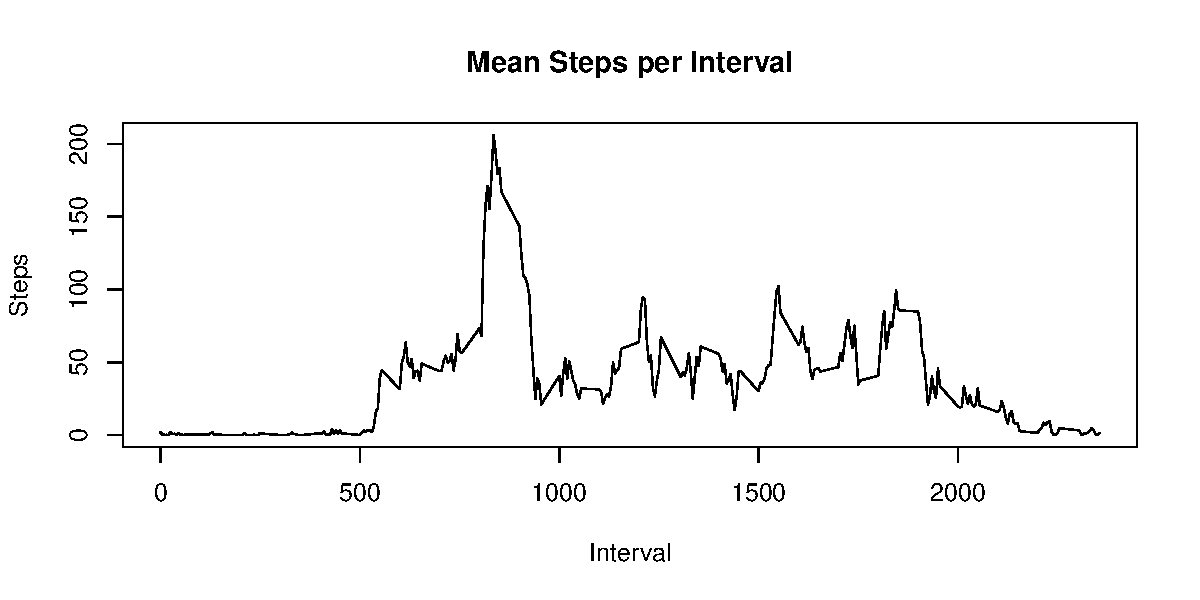
\includegraphics{PA1_template_files/figure-latex/unnamed-chunk-5-1.pdf}

\begin{Shaded}
\begin{Highlighting}[]
\CommentTok{#avg.int <- as.data.frame(cbind(rownames(avg.int),avg.int))}
\CommentTok{#colnames(avg.int) <- c("interval","steps")}

\NormalTok{maxint <-}\StringTok{ }\KeywordTok{which.max}\NormalTok{(avg.int$steps)}
\end{Highlighting}
\end{Shaded}

The interval with the maximum number of steps when averaged across all
days is \textbf{interval }.

\subsection{Imputing missing values}\label{imputing-missing-values-1}

\begin{Shaded}
\begin{Highlighting}[]
\NormalTok{narows <-}\StringTok{ }\NormalTok{raw.activity[!}\KeywordTok{complete.cases}\NormalTok{(raw.activity),]}
\NormalTok{rowcount <-}\StringTok{ }\KeywordTok{nrow}\NormalTok{(narows)}
\NormalTok{daycount <-}\StringTok{ }\KeywordTok{unique}\NormalTok{(narows$date)}
\end{Highlighting}
\end{Shaded}

There are \textbf{2304} rows with NAs in the dataset across ** r
daycount **

Replace missing values with the average for that interval on the missing
days

\begin{Shaded}
\begin{Highlighting}[]
\NormalTok{infna <-}\StringTok{ }\KeywordTok{merge}\NormalTok{(narows[, }\KeywordTok{c}\NormalTok{(}\StringTok{"date"}\NormalTok{, }\StringTok{"interval"}\NormalTok{)], avg.int, }\DataTypeTok{by =} \StringTok{"interval"}\NormalTok{)}
\NormalTok{infact <-}\StringTok{ }\KeywordTok{rbind}\NormalTok{(activity,infna)}
\NormalTok{steps <-}\StringTok{ }\KeywordTok{tapply}\NormalTok{(infact$steps, infact$date, sum)}
\KeywordTok{qplot}\NormalTok{(steps) +}\StringTok{ }\KeywordTok{geom_histogram}\NormalTok{(}\DataTypeTok{colour=}\StringTok{"black"}\NormalTok{, }\DataTypeTok{fill=}\StringTok{"grey"}\NormalTok{) +}\StringTok{ }
\StringTok{  }\KeywordTok{labs}\NormalTok{(}\DataTypeTok{x=}\StringTok{"Steps per day"}\NormalTok{, }\DataTypeTok{y=}\StringTok{"Frequency"}\NormalTok{, }\DataTypeTok{title=}\StringTok{"Histogram of Total Steps per Day with Missing Values Inferred"}\NormalTok{)}
\end{Highlighting}
\end{Shaded}

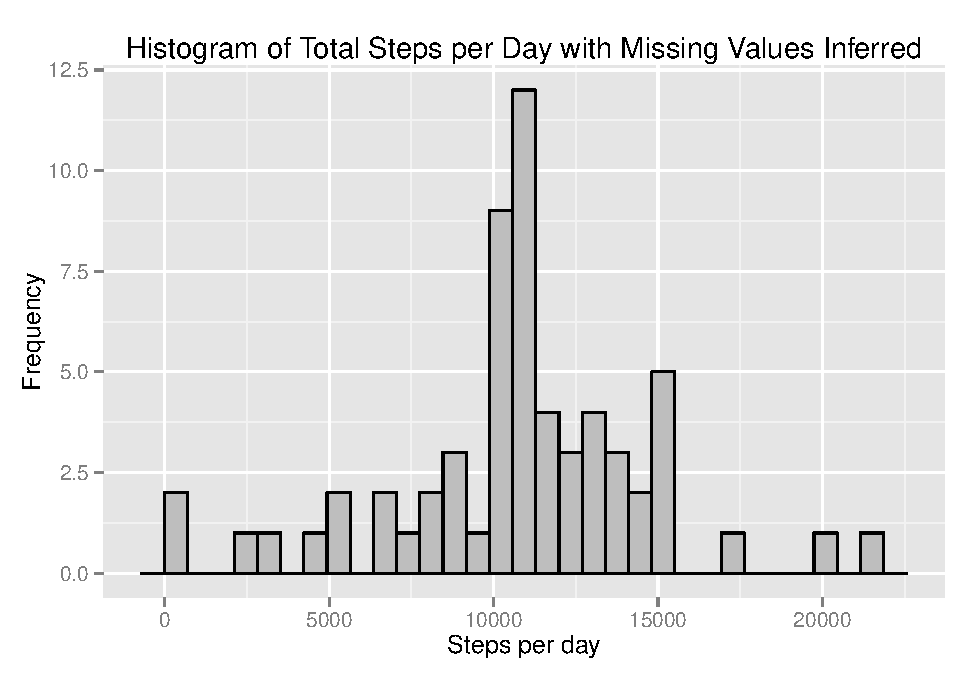
\includegraphics{PA1_template_files/figure-latex/unnamed-chunk-7-1.pdf}

\begin{Shaded}
\begin{Highlighting}[]
\NormalTok{mean.steps <-}\StringTok{ }\KeywordTok{mean}\NormalTok{(steps, }\DataTypeTok{na.rm=}\OtherTok{TRUE}\NormalTok{)}
\NormalTok{median.steps <-}\StringTok{ }\KeywordTok{median}\NormalTok{(steps, }\DataTypeTok{na.rm=}\OtherTok{TRUE}\NormalTok{)}
\end{Highlighting}
\end{Shaded}

\subsection{Are there differences in activity patterns between weekdays
and
weekends?}\label{are-there-differences-in-activity-patterns-between-weekdays-and-weekends-1}

\begin{Shaded}
\begin{Highlighting}[]
\NormalTok{infact$weekday <-}\StringTok{ }\KeywordTok{factor}\NormalTok{(}\KeywordTok{weekdays}\NormalTok{(}\KeywordTok{as.Date}\NormalTok{(infact$date)),}
                       \DataTypeTok{levels=}\KeywordTok{c}\NormalTok{(}\StringTok{"Sunday"}\NormalTok{, }\StringTok{"Monday"}\NormalTok{, }\StringTok{"Tuesday"}\NormalTok{, }\StringTok{"Wednesday"}\NormalTok{,}
                                \StringTok{"Thursday"}\NormalTok{, }\StringTok{"Friday"}\NormalTok{, }\StringTok{"Saturday"}\NormalTok{))}

\NormalTok{day.type <-}\StringTok{ }\KeywordTok{factor}\NormalTok{(infact$weekday %in%}\StringTok{ }\KeywordTok{c}\NormalTok{(}\StringTok{"Saturday"}\NormalTok{,}\StringTok{"Sunday"}\NormalTok{))}
\NormalTok{infact$day.type <-}\StringTok{ }\KeywordTok{mapvalues}\NormalTok{(day.type, }\DataTypeTok{from=}\KeywordTok{c}\NormalTok{(}\StringTok{"FALSE"}\NormalTok{, }\StringTok{"TRUE"}\NormalTok{), }\DataTypeTok{to=}\KeywordTok{c}\NormalTok{(}\StringTok{"Weekday"}\NormalTok{, }\StringTok{"Weekend"}\NormalTok{))}

\NormalTok{weekday.avg.int <-}\StringTok{ }\KeywordTok{ddply}\NormalTok{(infact, .(interval, day.type), summarise, }\DataTypeTok{steps=}\KeywordTok{mean}\NormalTok{(steps, }\DataTypeTok{na.rm=}\OtherTok{TRUE}\NormalTok{))}

\KeywordTok{ggplot}\NormalTok{(weekday.avg.int, }\KeywordTok{aes}\NormalTok{(interval, steps)) +}\StringTok{ }\KeywordTok{geom_line}\NormalTok{() +}\StringTok{ }\KeywordTok{facet_grid}\NormalTok{(day.type ~}\StringTok{ }\NormalTok{.) +}
\StringTok{    }\KeywordTok{labs}\NormalTok{(}\DataTypeTok{x=}\StringTok{"Interval"}\NormalTok{, }\DataTypeTok{y=}\StringTok{"Steps"}\NormalTok{, }\DataTypeTok{title=}\StringTok{"Activity by day type"}\NormalTok{)}
\end{Highlighting}
\end{Shaded}

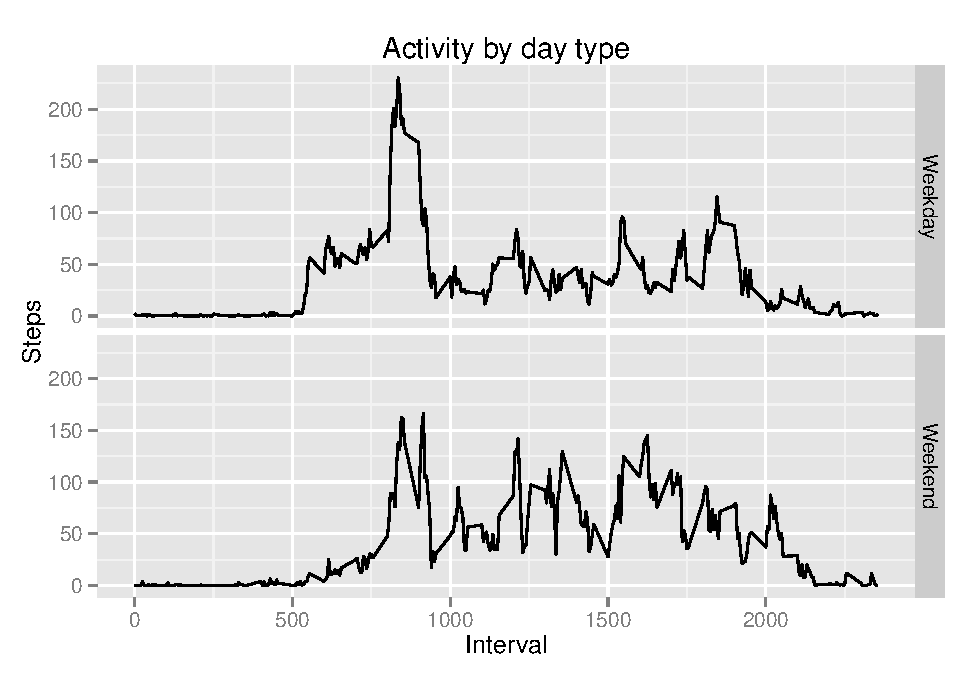
\includegraphics{PA1_template_files/figure-latex/unnamed-chunk-8-1.pdf}

\end{document}
